\chapter{Introducción}

En la historia de la humanidad surgen momentos y etapas que transcienden lo cotidiano y se convierten en hitos definitorios de una era. Uno de estos hitos que han marcado una etapa adversa en la historia moderna ha sido la pandemia de COVID-19, cuyos síntomas han afectado en cada rincón del planeta y han sacudido los cimientos de nuestra existencia de manera profunda. 

Cada uno de nosotros en cierta medida, hemos experimentado un crisol de emociones y desafíos que invitan a la introspección y la búsqueda de significado a la adversidad. La soledad ocasionada por el confinamiento y alejamiento de nuestras personas queridas, la ansiedad, la depresión y el estrés se volvieron parte del día a día de muchas personas.

En medio de todo este revuelo, la mente humana, enrevesada, reaccionó planteándose algunas preguntas existenciales ¿Qué valores importan en tiempos de crisis? ¿Cómo podemos encontrar la fortaleza para luchar contra la incertidumbre? 

Esto ha provocado que la población haya tenido que experimentar un periodo de adaptación a esta nueva normalidad. Ha habido un gran cambio en el desarrollo del cerebro de la población juvenil provocado por el confinamiento, la vulnerabilidad psicosocial y aumento a la exposición a las redes sociales que afectan a las habilidades socioemocionales, generando conductas de agresividad, falta de empatía, ansiedad, síntomas depresivos, dificultades para la resolución de conflictos\textit{(\cite{psychiatry2020})}. 

Y no solo en este sentido, ya que el bienestar se refiere a un estado general de satisfacción y equilibrio en la vida y se compone de varios aspectos, como la salud física, la salud mental, la calidad de vida y el sentido de propósito y conexión con los demás\textit{(\cite{bienestar})}. Por lo que debemos tener en cuenta que el bienestar no es un aspecto individual, sino que se encuentra asociado al entorno en el que vivimos y que nos ayuda a hacer frente a los factores estresantes de la vida, a aprender y trabajar bien, y a contribuir a nuestra comunidad. \vspace{0.3cm}

En definitiva, la importancia del bienestar se ha vuelto crucial, ya que la pandemia ha afectado significativamente a la calidad de vida de las personas. Es esencial abordar el bienestar como una cuestión de interés público y trabajar juntos para construir una sociedad más saludable y equitativa. \\[3cm]

\begin{figure}[!ht]
    \centering
    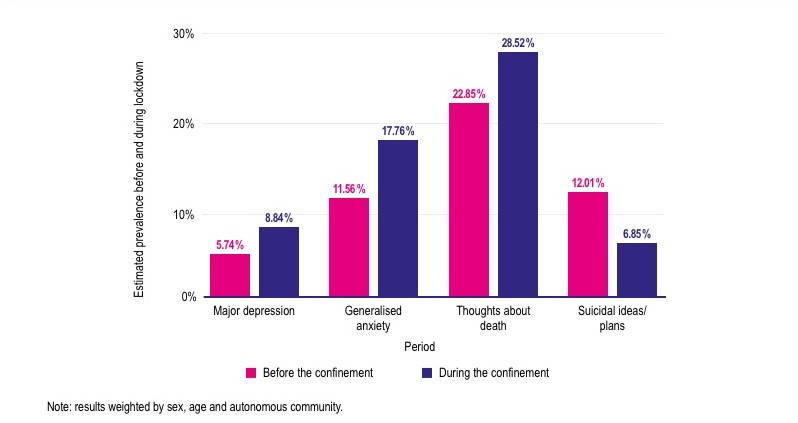
\includegraphics[width=1\textwidth]{imagenes/graficaCovid.jpg}
    \caption{ Comparación de personas con problemas mentales antes y durante la pandemia por\textit{(\cite{impactocovid})}}
    \label{fig:enter-label}
\end{figure}


\section{Motivación}

La nueva normalidad socioeconómica tras el brote de COVID-19 plantea desafíos sin precedentes tanto para los gobiernos como para los ciudadanos. Desde el inicio de la pandemia los gobiernos han tenido acceso a diversos datos económicos, pero la información precisa sobre cómo la nueva normalidad y las políticas específicas influyen en la conducta individual y grupal y, en consecuencia, en el bienestar de la sociedad, es escasa, indirecta y abierta a la interpretación. Como argumenta \textit{(\cite{medicion2009})} son necesarios datos que proporcionen un indicador cuantitativo confiable de cómo las diferentes medidas y su impacto en el contexto económico, social y conductual afectan el bienestar general de la población.\vspace{0.3cm}

Gracias al uso masivo de teléfonos inteligentes podemos recoger datos ubicuos, continuos y anónimos de la población, así como datos emocionales, sociales, conductuales y relativos al bienestar.\vspace{0.3cm}

En este contexto, la creación de un agente conversacional en \href{https://telegram.com.es/}{\textit{(Telegram)}} se nos presenta como una ingeniosa solución para esta recolección de datos. La motivación de de este proyecto radica en la importancia de poder brindar al usuario un espacio confidencial y seguro a través de conversaciones interactivas y personalizadas para que las personas puedan expresar sus emociones sin ningún tipo de pensamiento crítico.
Además Telegram consta de un diseño atractivo permitiendo la integración de cuestionarios, encuestas, enlaces,lo que facilita el acceso a recursos de apoyo\vspace{0.3cm}

Toda esta información recogida puede ser muy útil para investigadores, profesionales del sector, ya que proporcionan una visión más precisa de las necesidades y desafíos a los que enfrenta los ciudadanos. 


\begin{quote}
    \textit{"De vez en cuando, una nueva tecnología, un antiguo problema y una gran idea se convierten en una innovación"} \\ 
    -- Dean Kamen. Creador del Segway y el iBOT.
\end{quote}

\section{Objetivos}

Este proyecto tiene como objetivo el desarrollo de un chatbot con el que recabar información personal sobre aspectos claves en el bienestar de las personas, de forma que nos permita clasificarla y estructurarla para generar un análisis. 

- Creación del chatbot para la recogida de datos relacionados con el bienestar.\vspace{0.1cm}

- Creación de una interfaz para comunicarnos con el chatbot. \vspace{0.1cm}

- Lógica interna propia del chatbot para adaptarse al contexto que estemos hablando y dar una respuesta digna. \vspace{0.1cm}

- Desarrollo de una aplicación web que nos permita interactuar con el chatbot y las preguntas a realizar.\vspace{0.1cm}

- Almacenamiento de las preguntas y respuestas en la base de datos de forma automática.
\vspace{0.3cm}

\section{Estructura}

En este primer capítulo hemos visto una introducción del proyecto, comentando la motivación del mismo y los objetivos a cumplir a lo largo de este desarrollo. En el segundo capítulo, nos pondremos un poco más en contexto y veremos ejemplos de chatbots en la actualidad relacionados con nuestro tema e intentaremos entender como funcionan, como nos ayudan y forman parte de nuestro día a día.

En el tercer y cuarto capítulo hablaremos sobre la planificación y etapas seguidas en el ciclo de vida del proyecto. Indagaremos en las tecnologías usadas, los requerimientos necesarios de nuestro trabajo, exponiendo las funcionalidades de todas las partes implicadas, problemas a abordar y como satisfacerlos. Seguidamente en los capítulos posteriores encontraremos toda la información necesaria para entender el desarrollo y la implementación del proyecto, para finalizar con la puesta a punto, conclusiones y aspectos a mejorar. 